\documentclass[tikz]{standalone}

\begin{document}


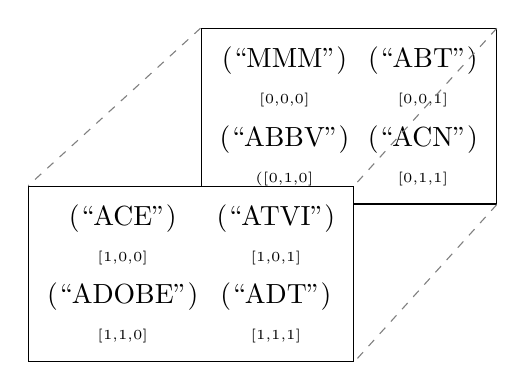
\begin{tikzpicture}
\def\xs{2} %shift in x direction
\def\ys{2} %shift in y direction
\def\nm{2} % number of 2d matrices in the 3d matrix


\matrix [draw, % for the rectangle border
         fill=white, % so that it is not transparent
         ampersand replacement=\&] %see explanation
(mm1)%give the matrix a name
at(-1* \xs, -1 * \ys) %shift the matrix
{
    \node {(``MMM'')}; \& \node {(``ABT'')};\\
	\node[font=\tiny] {[0,0,0]}; \& \node[font=\tiny] {[0,0,1]};\\
    \node {(``ABBV'')}; \& \node {(``ACN'')};\\
	\node[font=\tiny] {([0,1,0]}; \& \node[font=\tiny] {[0,1,1]};\\
};

\matrix [draw, % for the rectangle border
         fill=white, % so that it is not transparent
         ampersand replacement=\&] %see explanation
(mm2)%give the matrix a name
at(-2* \xs, -2 * \ys) %shift the matrix
{
    \node {(``ACE'')}; \& \node {(``ATVI'')};\\
	\node[font=\tiny] {[1,0,0]}; \& \node[font=\tiny] {[1,0,1]};\\
    \node {(``ADOBE'')}; \& \node {(``ADT'')};\\
	\node[font=\tiny] {[1,1,0]}; \& \node[font=\tiny] {[1,1,1]};\\
};
\draw [dashed,gray](mm1.north west) -- (mm\nm.north west);
\draw [dashed,gray](mm1.north east) -- (mm\nm.north east);
\draw [dashed,gray](mm1.south east) -- (mm\nm.south east);


\end{tikzpicture}


\end{document}
